%%%%%%%%%%%%%%%%%%%%%%%%%%%%%%%%%%%%%%%%%%%%%%%%%%%%%%%%%%%%%%%%%%%%%%%%%%%%%%%%
%2345678901234567890123456789012345678901234567890123456789012345678901234567890
%        1         2         3         4         5         6         7         8

%\documentclass[letterpaper, 10 pt, conference]{ieeeconf}  % Comment this line out if you need a4paper

\documentclass[a4paper, 10pt, conference]{ieeeconf}      % Use this line for a4 paper

\IEEEoverridecommandlockouts                              % This command is only needed if 


\overrideIEEEmargins                                      % Needed to meet printer requirements.

%In case you encounter the following error:
%Error 1010 The PDF file may be corrupt (unable to open PDF file) OR
%Error 1000 An error occurred while parsing a contents stream. Unable to analyze the PDF file.
%This is a known problem with pdfLaTeX conversion filter. The file cannot be opened with acrobat reader
%Please use one of the alternatives below to circumvent this error by uncommenting one or the other
%\pdfobjcompresslevel=0
%\pdfminorversion=4

% See the \addtolength command later in the file to balance the column lengths
% on the last page of the document

% The following packages can be found on http:\\www.ctan.org
\usepackage{graphicx}
\usepackage{amsmath} % assumes amsmath package installed
\usepackage{mathrsfs}
\usepackage{amssymb}
\usepackage{epstopdf}
\usepackage{bm}
\newtheorem{theorem}{Theorem}
\newtheorem{definition}{Definition}
\newtheorem{lemma}{Lemma}
\newtheorem{assumption}{Assumption}
\usepackage{cases}

\title{\LARGE \bf
Guiding vector field for moving path following with collision avoidance*
}


\author{Yinsong Qu$^{1}$   % <-this % stops a space
\thanks{*This work was not supported by any organization}% <-this % stops a space
\thanks{$^{1}$Yinsong Qu is with College of Intelligent Systems Science and Engineering, 
	University of Harbin Engineering University, Harbin 150001, P.~R.~China.
    (e-mail: qu13298110549@163.com)}%
}


\begin{document}



\maketitle
\thispagestyle{empty}
\pagestyle{empty}


%%%%%%%%%%%%%%%%%%%%%%%%%%%%%%%%%%%%%%%%%%%%%%%%%%%%%%%%%%%%%%%%%%%%%%%%%%%%%%%%
\begin{abstract}

In this paper, a control strategy is presented for unmanned aerial vehicles (UAVs) to follow a moving path with collision avoidance. This paper extends recent results in composite guiding vector field theory for static path following to moving path following, resulting in a composite course rate controller.  The smooth bump functions are introduced to combine the desired course angular velocities produced by path following vector and collision avoidance vector. Based on the proposed control scheme, the vehicle can follow the moving path while circumventing obstacles perfectly. Simulations results validate the effectiveness of the proposed method.

\end{abstract}
%%%%%%%%%%%%%%%%%%%%%%%%%%%%%%%%%%%%%%%%%%%%%%%%%%%%%%%%%%%%%%%%%%%%%%%%%%%%%%%%
\section{INTRODUCTION}

In recent years, with the requirement of unmanned aerial vehicles (UAVs) in different domains, ranging from environmental monitoring, search,and rescue to surveillance and reconnaissance, UAVs have gained great attention \cite{c1}. As a typical motion control scenario, path following controls a vessel to follow a predefined geometric path without any time constraints \cite{c2}. For path following control, the guidance, navigation and control (GNC) system is imperative, among which, automatic guidance of vehicles plays an important role in the path following control of UAVs. Based on the path information, the guidance system is used to produce the desired heading signals for control system to implement path following task \cite{c3}. This paper considers the guidance system design for an UAV to follow a moving path in the plane while avoiding stationary or moving obstacles.


There are many possible approaches have been proposed for the design of guidance system, such as line-of-sight (LOS) \cite{c4}--\cite{c7}, deep reinforcement learning (DRL) methods \cite{c8,c9}, guiding vector fields (GVF) \cite{c10}--\cite{c12}. LOS guidance method proposed in \cite{c4} and \cite{c5} need to calculate the shortest distance between unmanned surface vessel (USV) and the projection point of the vessel's position on path, so that, it requires that the desired path is an open curve. To overcome this limitation, a path variable, as an extra degree of freedom in the controller design, is introduced to propagate the path-tangential reference frame \cite{c6,c7}.  A new path-following and obstacle avoidance control strategy for mobile robots is proposed based on the RL algorithm, which simplifies the dimensionality of the environment state, ensuring that the mobile robot can achieve the optimal solution between path selection and obstacle avoidance actions \cite{c8}. A path-following
control strategy based on a DDPG-based guidance law and an
ASMC is proposed for USV to follow geometric path in \cite{c9}. Among these geometrical path following methods, GVF method performs better than other guidance law. DRL control strategy need long-term training, but GVF method doesn't. It is shown that the GVF controller exhibit slower mean cross track error than LOS in \cite{c10}. The path following method is divided into carrot-chasing algorithm, NLGL, vector-field (VF)-based path following, LQR-based path following, and pure pursuit with LOS (PLOS)-based path following in \cite{c11}. and Monte Carlo simulations is utilized to validate that the vector field (VF) path-following technique more accurately follows the path than the other techniques and requires the least control effort. Therefore, vector field guidance method has great application prospect in path following and has attracted the research interest of many scholars. GVF guidance law for path following control is developed for straight-line paths and circular arcs or orbits in \cite{c12}. A time-varying GVF is proposed for USV to follow arbitrary curved paths in \cite{c13}, and uniform semiglobal exponential stability (USGES) proof is given by Lyapunov method.  It should be noted that the methods proposed in \cite{c12}--\cite{c14} are also limited by determining the shortest distance from a robot to the desired path. The guidance law proposed in \cite{c14,c15}, utilizing the level curve approach which does not employ any parametrization of path, is free of the computation of a projection of the robot posi-tion on the path. However, the desired path in the above methods is defined in the stationary frame, i.e., it does not contain time-varying items. There are also many applications that require vehicles to follow a desired path defined in the moving frame, such that, ground target tracking for UAV \cite{c16}, moving target enclosing for USV \cite{c17} or ground mobile robots \cite{c18}, etc. These tasks are also named as moving path following problem \cite{c21}. To compensate the time varying term included in the path, a guidance algorithm by expressing implicit equation of the desired path in the moving frame \cite{c19}. It should be noted that method in \cite{c19}  does not consider the collision avoidance problem, which is a crucial issue for safe navigation. Only a few studies focus on constructing vector field for following path with collision avoidance. In \cite{c20}, obstacles are modeled through Gaussian functions that modify the original function of path, generating a safe path, which is used to design a feedback controller, thus guaranteeing convergence to the path while avoiding all obstacles. In \cite{c21}, obstacle avoidance is incorporated into vector field guidance using repulsive vector fields and examines the effects of five different obstacle vector field decay functions on vehicle performance. An integrated path following and collision avoidance method using a composite vector field is proposed in \cite{c22}. The vector field for path following is integrated for collision avoidance via bump functions, which reduce significantly the overlapping effect. However, these methods doesn't consider the moving path following and collision avoidance simultaneously. The composite guiding vector method proposed in \cite{c22} cannot applying into moving path following directly.

Motivated by the considerations above, a new composite guidance law for moving path following control with collision avoidance is proposed in this paper. The main contributions of this paper are summarized as follows.

(1) Considering moving path following and collision avoidance simultaneously, we propose a composite guidance law to lead vehicle to follow a desired path while circumventing obstacles. The method proposed in \cite{c22} utilizes composite guiding vector to accom-plish path following task with collision avoidance. However, it does not consider the moving path following problem. The main difficult to get the composite guiding vector in this paper is that the vector fields used for moving path following and collision avoidance are not expressed in the same frame. The solution is to obtain desired course angular rates in {I} through these two vectors respectively, then composite them by the smooth bump functions.

(2) Since the information of obstacles is previously unknown, the collision-avoidance behavior is reactive for path following, which is practical for nautical navi-gation. The composite guidance law proposed in this paper considers the stationary and moving obstacles simultaneously, which can guarantee collision avoidance of stationary and moving obstacles reactively while leading the vehicle to approach to the desired moving path. 

The paper is organized as follows. The problem formulation is stated in Section II. The composite guidance law is given in Section III. Sec-tion IV shows the simulation results. At last, Section V concludes the paper.


\section{PROBLEM FORMULATION}

\subsection{Notations}

The notation $||\bm{\eta}||$ denote the norm of vector $\bm{\eta}\in \mathbb{R}^{n}$ and $\hat{\bm{\eta}}=\bm{\eta}/||\bm{\eta}||$ denote the standardization value $\bm{\eta}$. The desired path $\mathcal{P}$ is defined as $\mathcal{P}=\{\bm{\eta}\in \mathbb{R}^{\eta}:\phi(\bm{\eta})=0\}$, which is zeros-level set of the twice continuously differentiable function $\phi(\bm{\eta})$. We use $dist(\bm{p},\mathcal{P})$ to denote the Euclidean distance between $\bm{p}$ and $\mathcal{P}$, where $\bm{p}\in \mathbb{R}^{n}$ is a point in space. The symbol $dist(\bm{p}_1,\bm{p}_2)$ denote the Euclidean distance between two points $\bm{p}_1$ and $\bm{p}_2$. Assume $\bm{\eta} =[x,y]^T$. We use $\nabla \phi(\bm{\eta})$ to denote the gratitude of $\phi(\bm{\eta})$, $\nabla \phi(\bm{\eta})=[\partial \phi/\partial x,\partial \phi/\partial y]^T$. The notation $I_{n}$ represent an n-dimensional identity matrix. The notation $R(\psi)$ denote the rotation matrix with rotation angle $\psi$, $\bm{E}=R(90^{o})$ denote the special rotation matrix with rotation angle $90^{o}$ and $\bm{H}(\bm{\eta})$ denote Hessian matrix, which are defined as following.

\begin{equation}\label{eq1}
	\bm{R}(\psi)=
	\begin{bmatrix}
		\cos(\psi) & -\sin(\psi)\\
		\sin(\psi) & \cos(\psi)\\
	\end{bmatrix}
    \bm{E}=
	\begin{bmatrix}
		0 & -1\\
		1 & 0
	\end{bmatrix}
\end{equation}

\begin{equation}\label{eq2}
	\bm{H}(\bm{\eta})=
	\begin{bmatrix}
		\partial^{2} \phi/\partial^{2} x & \partial^{2} \phi/\partial x\partial y\\
		\partial^{2} \phi/\partial x\partial y & \partial^{2} \phi/\partial^{2} y\\
	\end{bmatrix}
\end{equation}

\subsection{Control Objective}

The kinematic model of UAV in the 2-D plane can be described as unicycletype
model:

\begin{equation}\label{eq3}
	\left\{
	\begin{aligned}
		\dot{\bm{\eta}}&=u\bm{m}+\bm{w}\\
		\dot{\psi}&=r
	\end{aligned}
	\right.
\end{equation}
where $\bm{\eta}=[x,y]^T$ is the position vector of UAV, $\bm{m}=[\cos(\psi),\sin(\psi)]^T$, $u$, $\psi$ and $r$ denotes the velocity, heading angle and angular velocity of UAV respectively, $\bm{w}$ denote the total disturbance.

In this paper, we consider the moving target enclosing problem, which can be also described as moving path following problem. Therefore, we need to obtain the path description in 2-D plane. Due to the motion of target, the establishment of frame $\{\mathcal{T}\}:XT-OT-YT$ is essential to describe desired path $\mathcal{P}$ (see Fig.~\ref{fig1}). For the sake of simplicity, we assume that the $\{\mathcal{T}\}$ is not rotational with respect to $\{\mathcal{I}\}: XI-OI-YI$, i.e., $\psi_T=0$. Let $\bm{\eta}_T=[x_T,y_T ]^T$ be the target position vector in $\{\mathcal{I}\}$. Then, the motion of target can be described in $\{\mathcal{I}\}$ as follows:

\begin{equation}\label{eq4}
	\dot{\bm{\eta}}_T=u_T\bm{m}_T
\end{equation}
where $\bm{m}_T=[\cos(\psi_T),\sin(\psi_T)]^T$, $u_T$ is the total speed of target. The position of UAV with respect to $\mathcal{T}$ can be defined in the following way:

\begin{equation}\label{eq5}
	\bm{\eta}_{pr}=\bm{R}(\psi_T)(\bm{\eta}-\bm{\eta}_T)
\end{equation}
where  is the rotational matrix characterizing the orientation of $\mathcal{T}$ with respect to $\mathcal{I}$. The desired path in $\mathcal{T}$ can be described by the zero-level set of an implicit function as follows:

\begin{equation}\label{eq6}
	\mathcal{P}=\{\bm{\eta}_{pr}\in \mathbb{R}^2:\phi(\bm{\eta}_{pr})=0\}
\end{equation}
where $\phi(\bm{\eta}_{pr}):\mathbb{R}^2\rightarrow \mathbb{R}$ is twice continuous differentiable. The description above does not require any parameterization. One can use the value $\phi(\bm{\eta}_{pr})$ to crudely represent the distance between the point $\bm{\eta}_{pr}$ and the desired path $\mathcal{P}$. This method need not find the nearest point in path to calculate shortest distance, so it is convenient in practical engineering. For simplicity, we named $\phi(\bm{\eta}_{pr})$ as path following error in frame $\{\mathcal{T}\}$. 

\begin{figure}[!htb]
	\centering
	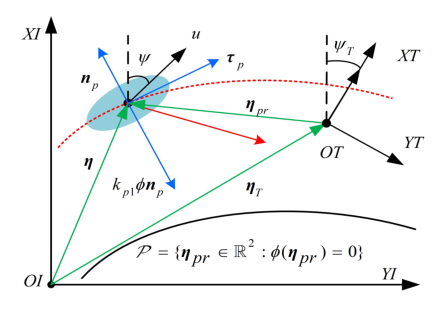
\includegraphics[width=8cm]{fig1.eps}
	\caption{Coordinated path following performance.}
	\label{fig1}
\end{figure}

In the process of enclosing the moving target, we often encounter various obstacles. To ensure navigation safety, we need to realize dynamic obstacle avoidance in the process of rounding up. We consider a finite set to describe the features of obstacles $\mathcal{O} =\{\mathcal{O} _i\subseteq \mathbb{R}^4,i\in I\}$, where $I\in \{1,2,...,n\}$ and n is the total number of obstacles, $\mathcal{O}_i=[x_{oi},y_{oi},R_{1i},R_{2i} ]^T$, in which, $x_{oi}$ and $y_{oi}$ represent the north and east position of ith obstacle respectively, the meaning of $R_{1i}$ and $R_{2i}$ will be discussed later. For convenience and intuition, we do not consider the specific geometry of the obstacle, but uniformly use circular curves to describe its outline. The circular curve can be expressed by the implicit function which is homeomorphic to a circle. Similar to [34], we define two different level sets to describe the reactive boundary $\mathcal{R}_i$ and repulsive boundary $\mathcal{Q}_i$ (see Fig 2) as 

\begin{equation}\label{eq7}
	\mathcal{R}_i=\{\bm{\eta}\in \mathbb{R}^2:\varphi(\bm{\eta})=0\}
\end{equation}
\begin{equation}\label{eq8}
	\mathcal{Q}_i=\{\bm{\eta}\in \mathbb{R}^2:\varphi(\bm{\eta})=c_i\}
\end{equation}
where $c_i\neq 0$ is a constant and $\varphi_i$ is a twice continuous differential function. Let the $R_{1i}$ and $R_{2i}$ represent radius of reactive and repulsive boundary respectively, $R_{1i}\leq R_{2i}$. As shown in Fig.~\ref{fig2}, the reactive boundary and the repulsive boundary divided the 2-D plane into three subsets, the first is named as safe area denoted by $^{ex}\mathcal{R}_i$ (the symbol "ex" represents "exterior"), the second is named as reactive area denoted by $^{in}\mathcal{R}_i\cap^{ex}\mathcal{Q}_i$ (the symbol "in" represents "interior"), and the third is named as repulsive area denoted by $^{in}\mathcal{Q}_i$. As mentioned earlier, we can use $\varphi_i$ to represent the distance between the point $\bm{\eta}$ and the center position of obstacle, i.e., the center position of reactive or repulsive area. Then, the value of $\varphi_i$ can be used to determine the area where the UAV is located at the current time, i.e., there are $\eta\in^{ex}\mathcal{R}_i$, if $\varphi_i\leq0$, $\bm{\eta}\in^{in}\mathcal{R}\cap^{ex}\mathcal{Q}_i$, if $c_i<\varphi_i<0$, $\bm{\eta}_i\in^{in}\mathcal{Q}_i$, if $\varphi_i\leq c_i$.

\begin{figure}[!htb]
	\centering
	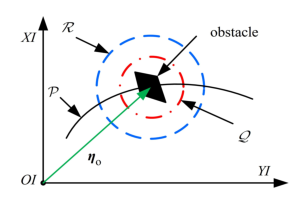
\includegraphics[width=7cm]{fig2.eps}
	\caption{Coordinated path following performance.}
	\label{fig2}
\end{figure}

From the discussion above, the control objectives can be described as: design a guiding vector filed to accom-plish the path following task while ensuring the naviga-tion safety. Detailed descriptions of objectives are given as follows:

O1)	(bounded path following error): there exists $M>0$ such that the path following error $|\phi(\bm{\eta}_{pr})|\leq M$ for $t\geq 0$, and the error function $|\phi(\bm{\eta}_{pr})|$ will decrease in the continuous time interval $t\in \Xi$ satisfying that $\phi (\bm{\eta}_{pr})\in^{ex}\mathcal{R}_i$.

O2)	(collision avoidance): for every initial position $\bm{\eta} (0)\in^{in}\mathcal{Q}_i$, there always exists a $T$ satisfying that $\bm{\eta}(t)\notin^{in}\mathcal{Q}_{i}$, when $t\geq T$; for every initial position $\bm{\eta}(0)\notin^{in}\mathcal{Q}_i$, then there is $\bm{\eta} (t)\notin^{in}\mathcal{Q}_i$ for all $t\in \mathbb{R}$. In addition, if there exists a time $t=t_1$ satisfying $\bm{\eta} (t_1)\in^{in}\mathcal{R}_i\cap^{ex}\mathcal{Q}_i$, then there must exist a time $t=t_2 (t_2>t_1)$ satisfying that $\bm{\eta} (t_2)\notin^{in}\mathcal{R}_{1i}\cap^{ex}\mathcal{Q}_{2i}$.

\subsection{Assumptions}
\begin{definition}
	The critical sets of curve path and repulsive boundary defined in (15) and (17) are denoted $C_P$ and $C_R$ respectively, and are defined as follows
	
	\begin{equation}\label{eq9}
		\mathcal{C}_P=\{\bm{\eta}_{pr}\in\mathbb{R}^2:\nabla \phi(\bm{\eta}_{pr})=0\}
	\end{equation}
	\begin{equation}\label{eq10}
		\mathcal{C}_R=\{\bm{\eta}\in\mathbb{R}^2:\nabla 	\phi(\bm{\eta}_{pr})=0\} 
	\end{equation}
	
\end{definition}

\begin{assumption}\label{as1}
	There exists two constants $\iota_1,\iota_2>0$ satisfying that 
	\begin{equation}\label{eq11}		
		\inf{\{|\nabla \phi(\bm{\eta}_{pr})|:\rm{dist}(\bm{\eta}_{pr},\mathcal{P})\leq\iota_1\}}>0
	\end{equation}
	\begin{equation}\label{eq12}
		\inf{\{|\nabla \phi(\bm{\eta})|:\rm{dist}(\bm{\eta},\mathcal{R})\leq\iota_2\}}>0
	\end{equation}
\end{assumption}

\begin{assumption}\label{as2}
	 Any two obstacles are sufficiently far away from each other, so that the any two obstacles reactive areas are disjoint, i.e., there holds $\rm{dist}$$(\bm{P}_i,\bm{P}_j )>0$, where $\bm{P}_i\in^{in}\mathcal{R}_i$ , $\bm{P}_j\in^{in}\mathcal{R}_j$.
\end{assumption}

\emph{Remark 1:}
	 Assumption 1 means that the sets of critical points $\mathcal{C}_P$ and $\mathcal{C}_R$ are separated from path P and repulsive boundary R by a positive distance $\rm{dist}(\bm{\eta}_{pr},\mathcal{P})\leq\iota_1$ and $\rm{dist}(\bm{\eta},\mathcal{R})\leq\iota_2$, where $\iota_1, \iota_2>0$, respectively. Assumption 2 is reasonable for the description of obstacles. If the adjacent obstacles are too close, we can use a larger reaction domain to describe, rather than separate a single description, which is practical and simplifies the obstacle avoidance problem.

\section{MAIN RESULT}

This section is divided into three parts, the vector field for moving path following is designed in part A, the vector field for collision avoidance is designed in part B, then, the switching of the above two vector fields is completed by introducing switching function in part C, and the design of composite guidance law is also realized. The properties of the solutions are given in part D. 

\subsection{Moving path following guidance law} 
Let $\bm{m}_{pr}=\bm{R}^T (\psi_T)(u\bm{m} +\bm{w}-u_T\bm{m}_T)$, there are $\bm{m}_{pr}=\dot{\bm{\eta}}_{pr}$ and $\dot{\bm{m}}_{pr}=\ddot{\bm{\eta}}_{pr}$. The intuitive meaning of $\bm{m}_{pr}$ is the velocity vector of $\bm{\eta}_{pr}$ with respect to $\{\mathcal{T}\}$. As above, we normalize $\bm{m}_{pr}$ to $\hat{\bm{m}}_{pr}$, then, (\ref{eq3}) can be rewrite as:

\begin{equation}\label{eq13}
	\dot{\bm{\eta}}_{pr}=||\bm{m}_{pr}||\hat{\bm{m}}_{pr}
\end{equation}

Then, the 2-D target enclosing vector field can be given as the following combination form:

\begin{equation}\label{eq14}
	\bm{m}_{pd}=\bm{\tau}_{p}-k_{p1}\phi(\bm{\eta}_{pr}) \bm{n}_p
\end{equation}
where $\bm{n}_p=\nabla \phi(\bm{\eta}_{pr})$, $\bm{\tau}_p=\bm{E}\bm{n}_p$, $k_{p1}>0$. Next, our main task is to design a guidance law $r_{pd}$ ensuring that $\bm{m}_{pr}\rightarrow \bm{m}_{pd}$, if $r\rightarrow r_{pd}$. $\dot{\psi}_{pd}$ is calculated as

\begin{equation}\label{eq15}
	\left\{
	\begin{aligned}
		\dot{\hat{\bm{m}}}_{pr}&=-\frac{1}{||\bm{m}_{pr}||}E\hat{\bm{m}}_{pr}\hat{\bm{m}}^T_{pr}\bm{E}\dot{\bm{m}}_{pr}\\
		\dot{\bm{m}}_{pr}&=ur\bm{R}^T(\psi_T)\bm{E}\bm{m}
	\end{aligned}
	\right.
\end{equation}

Since $\hat{\bm{m}}_{pd}$ is a normalization vector, we can expressed it into the following form, $\hat{\bm{m}}_{pd}=[\cos(\psi_{pd}),\sin(\psi_{pd})]^T$, where $\psi_{pd}$ is the orientation angle of vector $\hat{\bm{m}}_{pd}$. The derivative of $\hat{\bm{m}}_{pd}$ is calculated by

\begin{equation}\label{eq16}
	\dot{\hat{\bm{m}}}_{pd}=\dot{\psi}_{pd}\bm{E}\hat{\bm{m}}_{pd}
\end{equation}
where $\dot{\psi}_{pd}$ is calculated as

\begin{equation}\label{eq17}
	\left\{
	\begin{aligned}
		\dot{\psi}_{pd}&=-\hat{\bm{m}}^T_{pd}\bm{E}\dot{\hat{\bm{m}}}_{pd}\\
		\dot{\hat{\bm{m}}}_{pd}&=-\frac{1}{||\bm{m}_{pd}||}E\hat{\bm{m}}_{pd}\hat{\bm{m}}^T_{pd}\bm{E}\dot{\bm{m}}_{pd}\\
		\dot{\bm{m}}_{pd}&=-k_{p1}\bm{n}^T_p\dot{\bm{\eta}}_{pr}\bm{n}_p+(E-k_{p1}\phi \bm{I}_2)\bm{H}\dot{\bm{\eta}}_{pr}
	\end{aligned}
	\right.
\end{equation}

Let $e_{p}=\hat{\bm{m}}_{pr}-\hat{\bm{m}}_{pd}$, then the Lyapunov candidate function can be chosen as $V_{p1}=0.5e^T_{p}e_p$. Combining with (\ref{eq14})--(\ref{eq16}), the derivative of $V_{p1}$ can be calculated as

\begin{equation}\label{eq18}
	\begin{aligned}
		\dot{V}_{p1}&=(\hat{\bm{m}}_{pr}-\hat{\bm{m}}^T_{pd})(\dot{\hat{\bm{m}}}_{pr}-\dot{\hat{\bm{m}}}_{pd})\\
		&=-\frac{ur}{||\bm{m}_{pr}||}\hat{\bm{m}}^T_{pr}E\hat{\bm{m}}_{pr}\hat{\bm{m}}^T_{pr}R^T(\psi_T)\bm{m}-\dot{\psi}_{pd}\hat{\bm{m}}^T_{pr}\bm{E}\hat{\bm{m}}_{pd}\\
		&=-(\frac{ur}{||\bm{m}_{pr}||}\hat{\bm{m}}^T_{pr}\bm{R}^T(\psi_T)\bm{m}-\dot{\psi}_{pd})\hat{\bm{m}}^T_{pr}\bm{E}\hat{\bm{m}}_{pd}
	\end{aligned}
\end{equation}

Then, the guidance law is given as

\begin{equation}\label{eq19}
	r_{pd}=\frac{||\bm{m}_{pr}||(\dot{\psi}_{pd}-k_{p2}\hat{\bm{m}}^T_{pr}\bm{E}\hat{\bm{m}}_{pd})}{u\hat{\bm{m}}^T_{pr}\bm{R}^T(\psi_T)\bm{m}}
\end{equation}

\subsection{Collision Avoidance guidance law}

Let $\bm{m}_c=u\bm{m}+\bm{w}$. The kinematic model of UAV expressed in (\ref{eq3}) can be rewrite as:

\begin{equation}\label{eq20}
	\dot{\bm{\eta}}=||\bm{m}_{c}||\hat{\bm{m}}_{c}
\end{equation}

To simplify symbol description, we only consider one existing obstacle, then, the subscript $i$ in (\ref{eq8}), (\ref{eq9}) can be omitted. From the definition of reactive boundary in (\ref{eq8}), we can define the vector field for collision avoidance as follows:

\begin{equation}\label{eq21}
	\bm{m}_{od}=\bm{\tau}_{o}-k_{o1}\varphi(\bm{\eta}) \bm{n}_o
\end{equation}
where $\bm{n}_o=\nabla \varphi(\bm{\eta})$, $\bm{\tau}_o=\bm{E}\bm{n}_o$, $k_{o1}>0$. We can easily get the derivative of $\bm{m}_c$ as

\begin{equation}\label{eq22}
	\left\{
	\begin{aligned}
		\dot{\hat{\bm{m}}}_{c}&=-\frac{1}{||\bm{m}_{c}||}\bm{E}\hat{\bm{m}}_{c}\hat{\bm{m}}^T_{c}\bm{E}\dot{\bm{m}}_{c}\\
		\dot{\bm{m}}_{c}&=ur\bm{E}\bm{m}
	\end{aligned}
	\right.
\end{equation}

Similar as, we have $\dot{\hat{\bm{m}}}_{od}=\dot{\psi}_{od}\bm{E}\hat{\bm{m}}_{od}$. Let $\bm{e}_o=\hat{\bm{m}}_{c}-\hat{\bm{m}}_{od}$. The Lyapunov function can be chosen as $V_{o2}=0.5\bm{e}^T_o\bm{e}_o$, its derivative is

\begin{equation}\label{eq23}
	\dot{V}_{o1}=(\frac{ur}{||\bm{m}_c||}\hat{\bm{m}}^T_c\bm{m}-\dot{\psi}_od)\hat{\bm{m}}^T_cE\hat{\bm{m}}_{od}
\end{equation}

Then, the guidance law is designed as

\begin{equation}\label{eq24}
	r_{od}=\frac{||\bm{m}_c||(\dot{\psi}_o-k_{o2}\hat{\bm{m}}^T_c\bm{E}\hat{\bm{m}}_{od})}{u\hat{\bm{m}}^T_c\bm{m}}
\end{equation}
where $\dot{\psi}_{od}$ is given as

\begin{equation}\label{eq25}
	\left\{
	\begin{aligned}
		\dot{\psi}_{od}&=-\hat{\bm{m}}^T_{od}\bm{E}\dot{\hat{\bm{m}}}_{od}\\
		\dot{\hat{\bm{m}}}_{od}&=-\frac{1}{||\bm{m}_{od}||}\bm{E}\hat{\bm{m}}_{od}\hat{\bm{m}}^T_{od}\bm{E}\dot{\bm{m}}_{od}\\
		\dot{\bm{m}}_{od}&=-k_{o1}\bm{n}_{o}^T\dot{\bm{\eta}}\bm{n}_o+(E-k_{o1}\phi \bm{I}_2)\bm{H}\dot{\bm{\eta}}
	\end{aligned}
	\right.
\end{equation}

Let $r=r_{od}$ and bring it into equation (\ref{eq23}), there is
 
\begin{equation}\label{eq26}
	\dot{V}_{o1}=-k_{o2}(\hat{\bm{m}}^T_c\bm{E}\hat{\bm{m}}_{od})^2
\end{equation}

\subsection{Composite guidance law}

Both the moving path following guidance law and the obstacle avoidance guidance law have been designed. In this part, the cut-in and cut-out function will be designed to realize the smooth switching of the two guidance law. 

The main idea for synthesis problem is to distribute different weights to the two-guidance law according to the distance between UAV and the center of the obstacle \cite{c22}. The weight is designed as a function of the distance from the center of the obstacle, and the weight changes continuously. So that when the UAV is outside the reactive boundary, i.e., it only conducts path follow-ing guidance law, the weight for path tracking guidance law is 1 while the weight of obstacle avoidance is 0; when entering the obstacle reactive area, it needs to conduct obstacle avoidance guidance and path tracking guidance at the same time, the weight function changes with the distance, so that the closer the distance from the center of the obstacle, the greater the weight of the obstacle avoidance guidance law, while, the path tracking guidance law weight decreases with the distance; when entering the obstacle repulsive area (high-risk area), the obstacle avoidance is the unique task, so that, the path tracking weight is 0 and the obstacle avoidance weight is 1. From the above analysis, the composite guidance law can be designed as:

\begin{equation}\label{eq27}
	r_d=\begin{cases}
		r_{pd},&\mbox{if}~\varphi(\bm{\eta})\leq c\\
		S_p r_{pd}+S_o r_{od},&\mbox{if}~c<\varphi(\bm{\eta})<0\\
		r_{od},&\mbox{if}~\varphi(\bm{\eta})\geq 0
	\end{cases}
\end{equation}
where the $S_p$ and $S_o$ represent the different weights, satisfying that $S_p+S_o=1$, then, $S_p$ and $S_o$ can be defined as:

\begin{equation}\label{eq28}
	S_p=\frac{f_p}{f_p+f_o},S_o=\frac{f_o}{f_p+f_o}
\end{equation}
where $f_p$ and $f_o$ are cut-in and cut-out function. $S_p$ should be positively correlated with the distance from the obstacle repulsive boundary, and $S_o$ should be positively correlated with distance from obstacle reactive boundary. The distance from obstacle reactive boundary and repulsive boundary can be calculated as $d_R=\varphi(\bm{\eta})-c$, $d_Q=-\varphi(\bm{\eta})$, respectively, where $c<\varphi(\bm{\eta})<0$. then, cut-in and cut-out function can be designed as follows \cite{c22}:

\begin{equation}\label{eq29}
	f_p=\exp{(-\frac{l_p}{d_R})},f_o=\exp{(-\frac{l_o}{d_Q})}
\end{equation}
where $l_p$ and $l_o$ are positive constants, determining the change rate of the cut in and cut out functions. Then, we give the function image of $f_p$ and $f_o$ with respect to $\varphi(\eta{\eta})$ in Fig 3, the parameter $l_p$ changes from 1 to 100, while another parameter $l_o$ remains unchanged. It is obvious that, with respect to same parameter $l_p$, the path following weight $S_p$ increase with the increase of $\varphi(\bm{\eta})$, which means UAV is further from obstacle, while collision avoidance weight $S_o$ increase with the decrease of $\varphi(\bm{\eta})$, which means UAV is closer to obstacle. Furthermore, it is worth noting that the bigger $l_p$ means the bigger $S_o$ is and the smaller $S_p$ with respect to same $\varphi(\bm{\eta})$. Therefore, we can tune the parameters $l_p$ and $l_o$ to change the priority of path following and collision avoidance. 

The composite guidance law is completed here. The convergent behaviors of the composite guidance law given in (\ref{eq27}) will be analysed in the next subsection.

\subsection{Properties of the solutions}

\begin{theorem}
	Applying the composite law proposed in (\ref{eq27}) into kinetics model (\ref{eq13}) and (\ref{eq20}), i.e., $r=r_d$, the trajectory of UAV expressed in $\{\mathcal{T}\}$ will converge to the desired moving path given by (\ref{eq6}) without bumping into the repulsive area $^{in}\mathcal{R}_{1i}$. 
\end{theorem}

\begin{proof}
According to the position of the UAV, the theorem will be divided into three parts.
	
case 1: Assuming $\bm{\eta}\in^{ex}\mathcal{R}_i$, there is only path following guidance law according to (\ref{eq27})-(\ref{eq29}), i.e., $r_d=r_{pd}$. Considering Lyapunov function as ,there will be $\bm{m}_{pr}\rightarrow \bm{m}_{pd}$. Acoording to the properties of $\bm{m}_{pd}$, $\phi(\bm{\eta}_{pr})$ will converge to the  small domain of 0, i.e., the trajectory of $\bm{\eta}_{pr}$ will converge to the  desired path $\mathcal{P}$ under the 
\emph{Assumption \ref{as1}} \cite{c23}.

case 2: Assuming $\bm{\eta}\in^{in}\mathcal{Q}_i$, there is only collision avoidance guidance law according to (\ref{eq27})-(\ref{eq29}), i.e., $r_d=r_{od}$. Considering Lyapunov function as ,there will be $\bm{m}_c\rightarrow \bm{m}_{od}$. Similar to the analysis of case 1, $\varphi(\bm{\eta})$ will converge to the  small domain of 0, i.e., the trajectory of $\bm{\eta}$ will converge to the  collision boundary $\mathcal{R}$ under the \emph{Assumption \ref{as1}}. 

case 3: Assuming $\bm{\eta}\in^{in}\mathcal{R}_i\cap ^{ex}\mathcal{Q}_i$, obstacle avoidance and following guidance law work at the same time, there is $r_d=S_or_{od}+S_pr_{pd}$. According to the properties of $S_p$ and $S_o$ given in (\ref{eq28}) and (\ref{eq29}), UAV will escape from the area $^{in}\mathcal{R}_i\cap ^{ex}\mathcal{Q}_i$ to the boundary $\mathcal{R}_{i}$. Back to the case 1, the UAV will following the desired path $\mathcal{P}$ after collision avoidance.

Based on case 1--case 3, we can conclude that the path following error $\phi(\bm{\eta}_{pr})$ is uniformly bounded.	
\end{proof}

\section{SIMULATIONS RESULTS}

To verify the effectiveness and widely serviceability of the proposed method, we conduct four groups simulations. In the case 1, the target is stationary, and there are obstacles occluding the desired path.In the case 2, the target is moving, and there exists obstacles.  

case 1:  (static path following with obstacles) Let $x_T=0$, $y_T=0$, $u_T=0$, $\psi_T=0$. In this case, we consider sinusoidal path described as $\phi(\bm{\eta}_{pr} )=y_{pr}^2-20\sin(?x_{pr}/25)$. The parameters for guidance law can be chosen as $k_{p1}=1$, $k_{p2}=1$, $k_{o1}=0.001$, $k_{o2}=0.5$. The obstacles are set as $O_1=[35,5,10,3]^T$ and $O_2=[65,-18,12,5]^T$. For bump function parameters, set parameter $l_o=1$ and $l_p=100$, respectively. Simulation time is set to 250s and simulation step is 0.02s. The simulation results are shown in Fig.~\ref{fig3} and Fig.~\ref{fig4}. As shown in Fig.~\ref{fig3} and Fig.~\ref{fig4}, all the trajectories can follow the desired path while avoiding obstacles perfectly,

\begin{figure}[!htb]
	\centering
	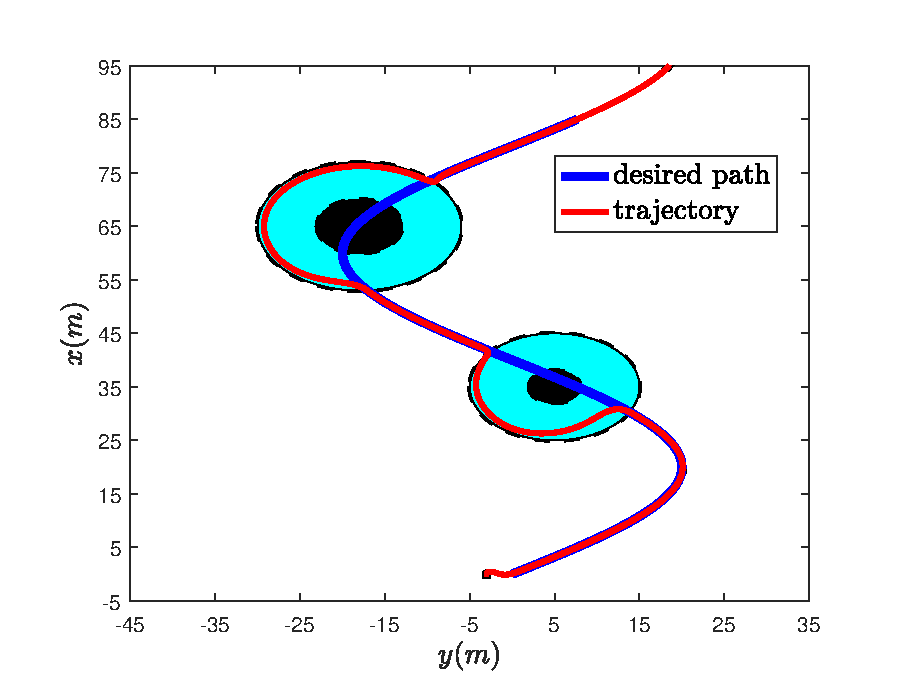
\includegraphics[width=\hsize]{case1_map.eps}
	\caption{Coordinated path following performance.}
	\label{fig3}
\end{figure}

\begin{figure}[!htb]
	\centering
	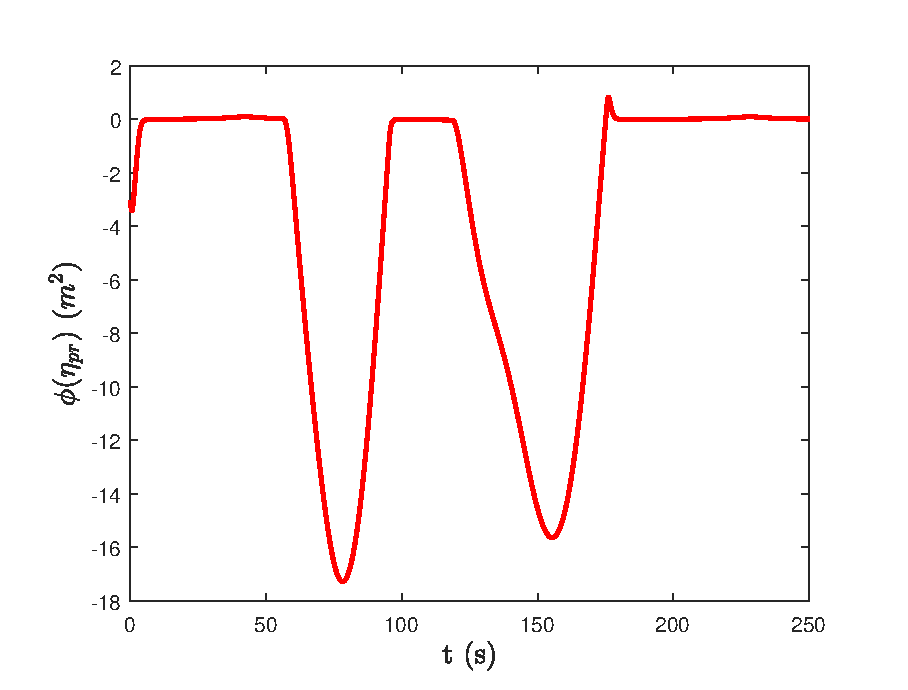
\includegraphics[width=\hsize]{case1_error.eps}
	\caption{Coordinated path following performance.}
	\label{fig4}
\end{figure}

case 2: (moving path following with obstacles) Let $x_T=0$, $y_T=0$, $u_T=0.3$, $\psi_T=0$. In this case, we consider the moving circular path defined as $\phi(\bm{\eta}_{pr})=x_{pr}^2+y_{pr}^2-36$ with the obstacles defined as $O_1=[30,20,8,3]^T$, $O_2=[40,50,6,2]^T$. The parameters for guidance law can be chosen as $k_{p1}=0.1$, $k_{p2}=1$, $k_{o1}=0.1$, $k_{o2}=1$, $l_p=100$, $l_o=1$. Simulation time is set to 450s and the simulation step is 0.02s. The simulation results are shown in Fig.~\ref{fig5} and Fig.~\ref{fig6}. As shown in Fig.~\ref{fig5}, UAV can enclose the target while avoiding obstacles. As shown in Fig.~\ref{fig6}, The path following error is bounded with obstacles, and will converge to zero without obstacles.

\begin{figure}[!htb]
	\centering
	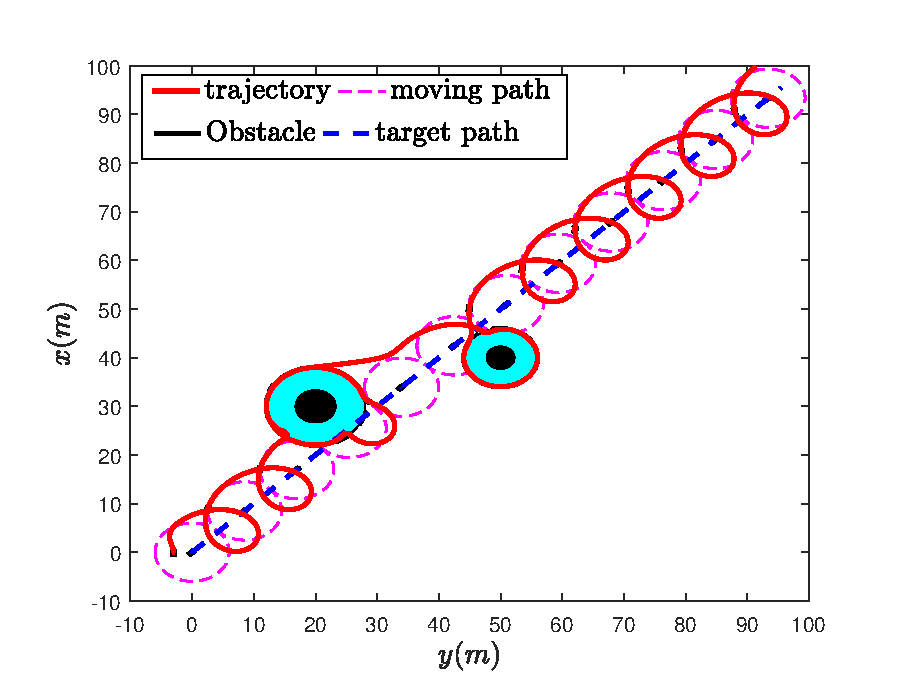
\includegraphics[width=\hsize]{case2_map.eps}
	\caption{Coordinated path following performance.}
	\label{fig5}
\end{figure}

\begin{figure}[!htb]
	\centering
	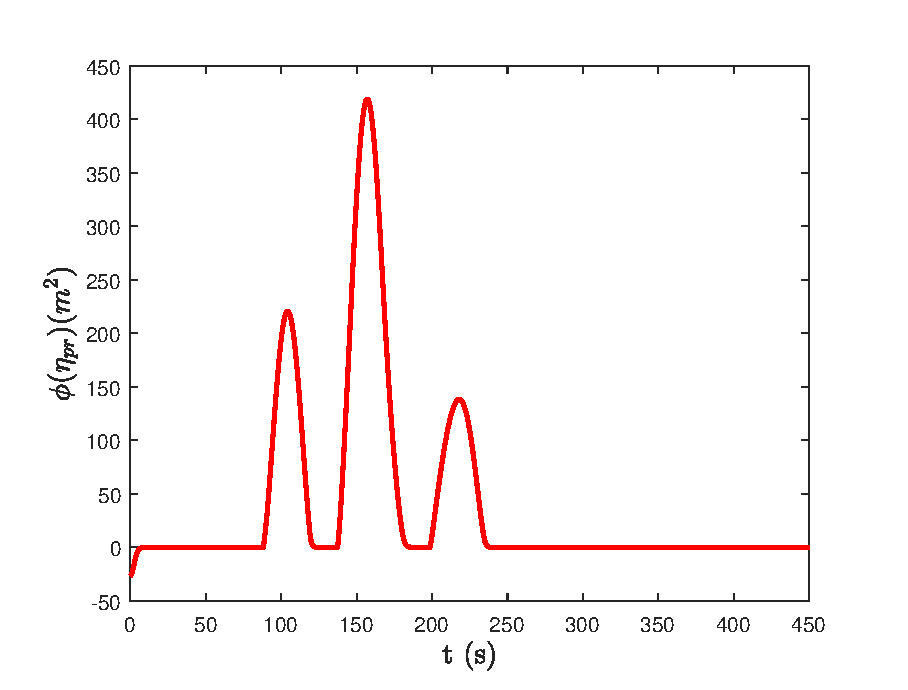
\includegraphics[width=\hsize]{case2_error.eps}
	\caption{Coordinated path following performance.}
	\label{fig6}
\end{figure}

\section{CONCLUSIONS}

In this paper, we propose a composite guidance law and control law for USV to follow a moving path with stationary obstacles avoidance, and provide elaborated stability analysis of the closed-loop system. This method can be used to solve the target enclosing, path following and target tracking problem for UAV moving in the 2-D palne or other 2-D mobile robots. The effectiveness and robustness of proposed method is validated by two groups of simulation experiments. The main disadvantages can be concluded into two points, the direction of obstacle avoidance cannot be determined effectively, the globally convergence to desired path is not guaranteed due to the critical points. We will solve these problem in the future works. We also plan to extend our method to cooperative moving path following for UAV with collision avoidance by guiding vector fields in the future work. 

\addtolength{\textheight}{-12cm}   % This command serves to balance the column lengths
                                  % on the last page of the document manually. It shortens
                                  % the textheight of the last page by a suitable amount.
                                  % This command does not take effect until the next page
                                  % so it should come on the page before the last. Make
                                  % sure that you do not shorten the textheight too much.

%%%%%%%%%%%%%%%%%%%%%%%%%%%%%%%%%%%%%%%%%%%%%%%%%%%%%%%%%%%%%%%%%%%%%%%%%%%%%%%%



%%%%%%%%%%%%%%%%%%%%%%%%%%%%%%%%%%%%%%%%%%%%%%%%%%%%%%%%%%%%%%%%%%%%%%%%%%%%%%%%



%%%%%%%%%%%%%%%%%%%%%%%%%%%%%%%%%%%%%%%%%%%%%%%%%%%%%%%%%%%%%%%%%%%%%%%%%%%%%%%%



%%%%%%%%%%%%%%%%%%%%%%%%%%%%%%%%%%%%%%%%%%%%%%%%%%%%%%%%%%%%%%%%%%%%%%%%%%%%%%%%



\begin{thebibliography}{99}

\bibitem{c1} Yang, J., Liu, C., Coombes, M., Yan, Y. and Chen, W.-H., “Optimal Path Following for Small Fixed-Wing UAVs Under Wind Disturbances”. \emph{IEEE Transactions on Control Systems Technology}, vol.29, no.3, pp.996--1008, 2020.
\bibitem{c2} Hung, N., Rego, F., Quintas, J., Cruz, J., Jacinto, M., Souto, D. et al., “A review of path following control strategies for autonomous robotic vehicles: Theory, simulations, and experiments”. \emph{Journal of Field Robotics}, 2022. 
\bibitem{c3} Xia, G., Wang, X., Zhao, B., Han, Z., Zheng, L., “Adaptive Neural Path Following Control of Underactuated Surface Vessels With Input Saturation”. \emph{IEEE Access}, vol.8, pp.92529--92540, 2020.
\bibitem{c4} Lekkas, A. M., Fossen, T. I., “Integral LOS Path Following for Curved Paths Based on a Monotone Cubic Hermite Spline Para-metrization”. \emph{IEEE Transactions on Control Systems Technology}, vol.22, pp.6, pp.2287--2301, 2014
\bibitem{c5} Fossen, T. I., Pettersen, K. Y., Galeazzi, R., “Line-of-Sight Path Following for Dubins Paths With Adaptive Sideslip Compensa-tion of Drift Forces”. \emph{IEEE Transactions on Control Systems Technology}, vol.23, no.2, pp.820--827, 2015.
\bibitem{c6} Belleter, D., Maghenem, M. A., Paliotta, C., Pettersen, K. Y., “Observer based path following for underactuated marine vessels in the presence of ocean currents: A global approach”. \emph{Automatica}, vol.100, pp.123--134, 2019.
\bibitem{c7} Bibuli, M., Caccia, M., Lapierre, L., Bruzzone, G., “Guidance of Unmanned Surface Vehicles: Experiments in Vehicle Following”. \emph{IEEE Robotics Automation Magazine}, vol.19, no.3, pp.92--102, 2012 
\bibitem{c8} Cheng, X.; Zhang, S.; Cheng, S.; Xia, Q.; Zhang, J, “Path-Following and Obstacle Avoidance Control of Nonholonomic Wheeled Mobile Robot Based on Deep Reinforcement Learning”. \emph{APPLIED SCIENCES-BASEL}, vol.12, no.14, 2022.
\bibitem{c9} A. Gonzalez-Garcia, H. Castaneda and L. Garrido, “USV Path-Following Control Based On Deep Reinforcement Learning and Adaptive Control”. in\emph{proceedings of Global Oceans 2020 Singapore U.S. Gulf Coast}, Biloxi, MS, USA, 2020: 1--7, 
\bibitem{c10} P. B. Sujit, S. Saripalli and J. B. Sousa, “Unmanned Aerial Vehicle Path Following: A Survey and Analysis of Algorithms for Fixed-Wing Unmanned Aerial Vehicless”. \emph{IEEE Control Systems Magazine}, vol. 34, no. 1, pp. 42--59, 2014.
\bibitem{c11} Caharija, W., Pettersen, K. Y., Calado, P., Braga, J., “A Comparison Between the ILOS Guidance and the Vector Field Guidance”. in \emph{proceedings of 10th IFAC Conference on Manoeuvring and Control of Marine Craft}, 2015: 89--94.
\bibitem{c12} Nelson, D. R., Barber, D. B., McLain, T. W., Beard, R. W., “Vector Field Path Following for Miniature Air Vehicles”. \emph{IEEE Transactions on Robotics}, vol.23, no.3, pp.519--529, 2007.
\bibitem{c13} Xu, H., Fossen, T. I., Soares, C. G., “Uniformly Semiglobally Exponential Stability of Vector Field Guidance Law and Autopilot for Path-Following”. \emph{European Journal of Control}, vol.53, pp.88--97, 2019.
\bibitem{c14} Liang, Y., Jia, Y., “Combined Vector Field Approach for 2D and 3D Arbitrary Twice Differentiable Curved Path Following with Constrained UAVs”. \emph{Journal of Intelligent Robotic Systems}, vol.83, no.1, pp.133--160, 2015.
\bibitem{c15} Yao, W., de Marina, H. G., Lin, B., Cao, M., “Singularity-Free Guiding Vector Field for Robot Navigation”. \emph{IEEE Transactions on Robotics}, vol.37, no.4, pp.1206--1221, 2021.
\bibitem{c16} Zhu, S., Wang, D., Low, C. B., “Ground Target Tracking Us-ing UAV with Input Constraints”. \emph{Journal of Intelligent Robotic Systems}, vol.69, no.1, pp.417--429, 2012.
\bibitem{c17} Z. Peng, Y. Jiang and J. Wang, “Event-Triggered Dynamic Surface Control of an Underactuated Autonomous Surface Vehicle for Target Enclosing”. \emph{IEEE Transactions on Industrial Electronics}, vol. 68, no. 4, 2021.
\bibitem{c18}	Yu, X., Liu, L., “Target Enclosing and Trajectory Tracking for a Mobile Robot With Input Disturbances”. \emph{IEEE Control Systems Letters}, vol.1, no.2, pp.221--226, 2017.
\bibitem{c19} Yuri A. Kapitanyuk, Hector Garcia de Marina, Anton V. Proskurnikov, Ming Cao, “Guiding vector field algorithm for a moving path follow-ing problem”, in \emph{proceedings of 20th World Congress of the International-Federation-of-Automatic-Control }, vol.50, no.1, pp.6983-6988, 2017.
\bibitem{c20} Tanveer, M. H., Recchiuto, C. T., Sgorbissa, A., “Analysis of path following and obstacle avoidance for multiple wheeled robots in a shared workspace”. \emph{Robotica}, vol.37, no.1,  pp.80--108, 2018.
\bibitem{c21} Wilhelm, J. P., Clem, G., “Vector Field UAV Guidance for Path Following and Obstacle Avoidance with Minimal Deviation”. \emph{Journal of Guidance, Control, and Dynamics}, vol.42, no.8, pp.1848--1856, 2019. 
\bibitem{c22} W. Yao, B. Lin, B. D. O. Anderson and M. Cao, “Guiding Vector Fields for Following Occluded Paths”. \emph{IEEE Transactions on Automatic Control}, vol. 67, no. 8, pp. 4091-4106, 2022.
\bibitem{c23} W. Yao, B. Lin, B. D. O. Anderson and M. Cao, “Topological Analysis of Vector-Field Guided Path Following on Manifolds”. \emph{IEEE Transactions on Automatic Control}, [Online]. 






\end{thebibliography}




\end{document}
